% 0L
\begin{figure}[h!]
    \centering
    \begin{subfigure}[b]{\textwidth}
        \centering
        \includegraphics[width=0.32\textwidth]{Images/VH/Own_fit/postfit_VHbb/Region_distmva_BMax600_BMin400_incFat1_Fat1_DSRnoaddbjetsr_J0_TTypebb_T2_L0_Y6051_GlobalFit_conditionnal_mu1.png
                                                                              Region_distmva_BMax600_BMin400_incFat1_Fat1_DSRnoaddbjetsr_J0_TTypebb_incJet1_T2_L0_Y6051_GlobalFit_conditionnal_mu1.png
        \includegraphics[width=0.32\textwidth]{Images/VH/Own_fit/postfit_VHbb/Region_distmva_BMax600_BMin400_incFat1_Fat1_DSRnoaddbjetsr_J1_TTypebb_incJet1_T2_L0_Y6051_GlobalFit_conditionnal_mu1.png}
        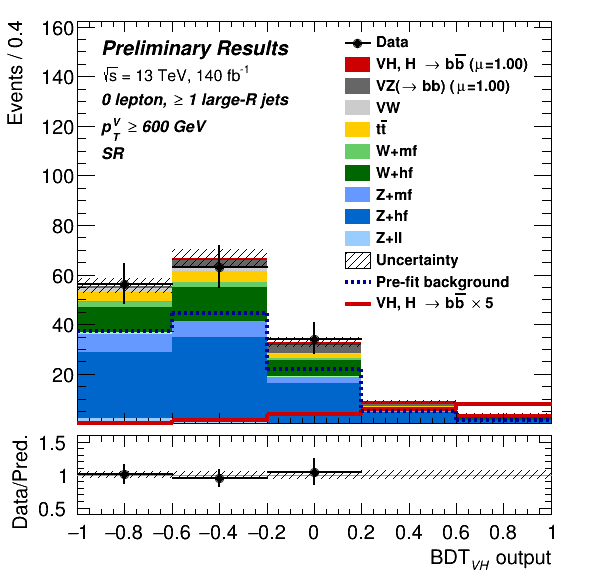
\includegraphics[width=0.32\textwidth]{Images/VH/Own_fit/postfit_VHbb/Region_distmva_BMin600_incFat1_Fat1_DSRnoaddbjetsr_J0_TTypebb_incJet1_T2_L0_Y6051_GlobalFit_conditionnal_mu1.png}
        \caption{The \ptv\ $\in$ [400, 600] GeV high- and low-purity (left and centre) and the \ptv\ $\geq$ 600 GeV (right) signal regions.}
        \label{fig:plots_VHbbBoost_OL_SR}
    \end{subfigure}
    \begin{subfigure}[b]{\textwidth}
        \centering
        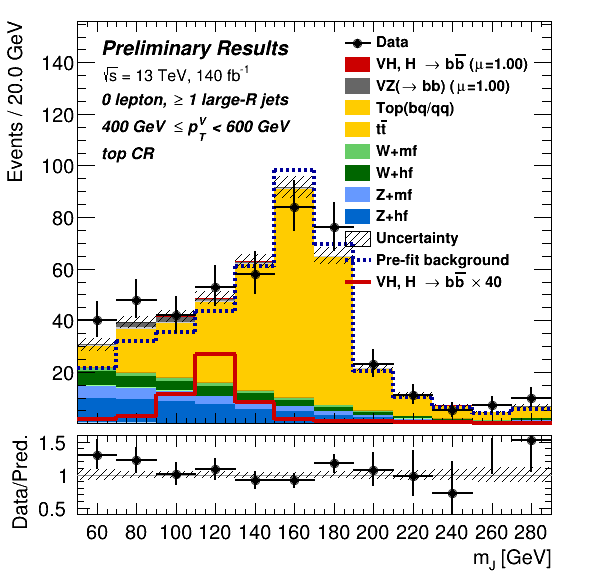
\includegraphics[width=0.32\textwidth]{Images/VH/Own_fit/postfit_VHbb/Region_distmBB_BMax600_BMin400_incFat1_Fat1_DSRtopaddbjetcr_J0_TTypebb_incJet1_T2_L0_Y6051_GlobalFit_conditionnal_mu1.png}
        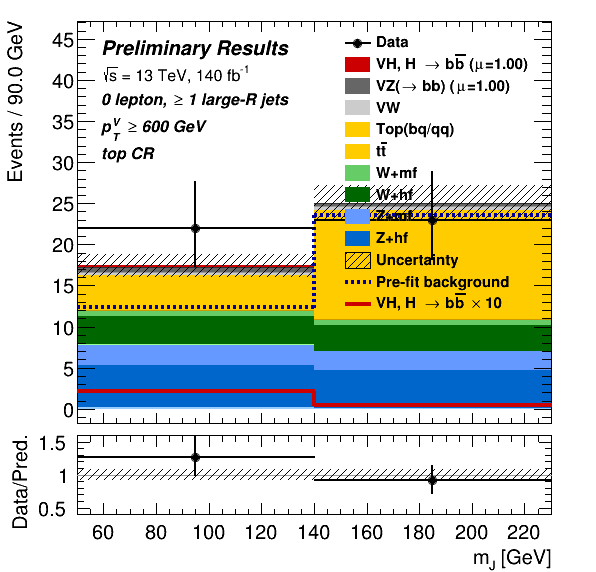
\includegraphics[width=0.32\textwidth]{Images/VH/Own_fit/postfit_VHbb/Region_distmBB_BMin600_incFat1_Fat1_DSRtopaddbjetcr_J0_TTypebb_incJet1_T2_L0_Y6051_GlobalFit_conditionnal_mu1.png}
        \caption{The \ptv\ $\in$ [400, 600] GeV (left) and \ptv\ $\geq$ 600 GeV (right) boosted Top CR.}
        \label{fig:plots_VHbbBoost_OL_topCR}
    \end{subfigure}
    \caption{The boosted $BB$-tagged 0L regions.}
    \label{fig:plots_VHbbBoost_OL}
\end{figure} 


% 1L

\begin{figure}[h!]
    \centering
    \begin{subfigure}[b]{\textwidth}
        \centering
        \includegraphics[width=0.32\textwidth]{Images/VH/Own_fit/postfit_VHbb/Region_distmva_BMax600_BMin400_incFat1_Fat1_DSRnoaddbjetsr_J0_TTypebb_T2_L1_Y6051_GlobalFit_conditionnal_mu1.png}
        \includegraphics[width=0.32\textwidth]{Images/VH/Own_fit/postfit_VHbb/Region_distmva_BMax600_BMin400_incFat1_Fat1_DSRnoaddbjetsr_J1_TTypebb_incJet1_T2_L1_Y6051_GlobalFit_conditionnal_mu1.png}
        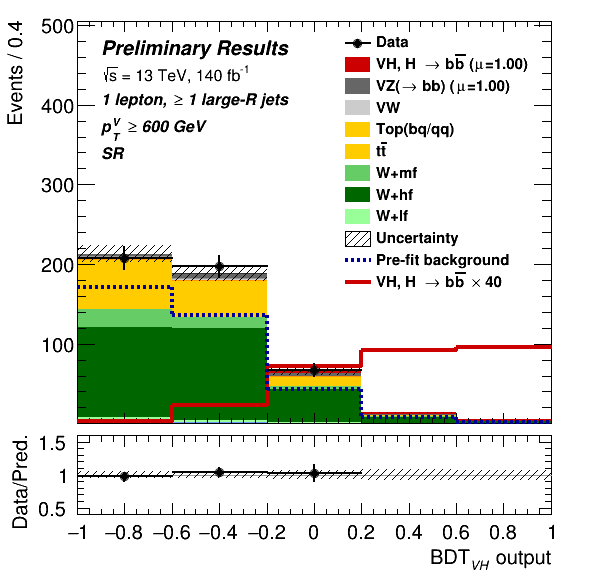
\includegraphics[width=0.32\textwidth]{Images/VH/Own_fit/postfit_VHbb/Region_distmva_BMin600_incFat1_Fat1_DSRnoaddbjetsr_J0_TTypebb_incJet1_T2_L1_Y6051_GlobalFit_conditionnal_mu1.png}
        \caption{The \ptv\ $\in$ [400, 600] GeV high- and low-purity (left and centre) and the \ptv\ $\geq$ 600 GeV (right) signal regions.}
        \label{fig:plots_VHbbBoost_1L_SR}
    \end{subfigure}
    \begin{subfigure}[b]{\textwidth}
        \centering
        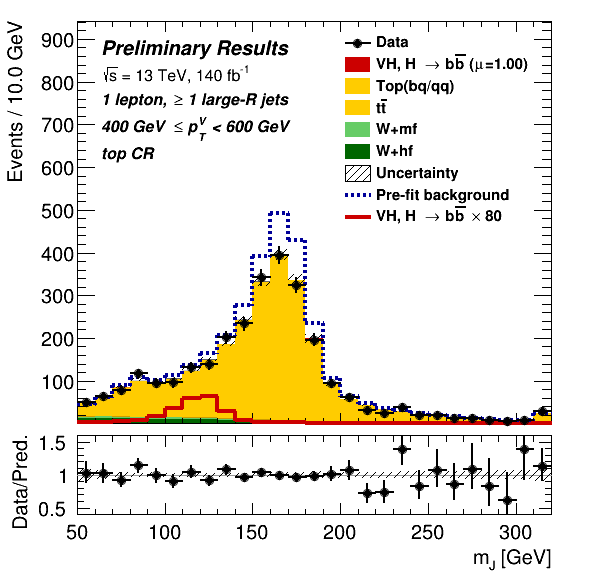
\includegraphics[width=0.32\textwidth]{Images/VH/Own_fit/postfit_VHbb/Region_distmBB_BMax600_BMin400_incFat1_Fat1_DSRtopaddbjetcr_J0_TTypebb_incJet1_T2_L1_Y6051_GlobalFit_conditionnal_mu1.png}
        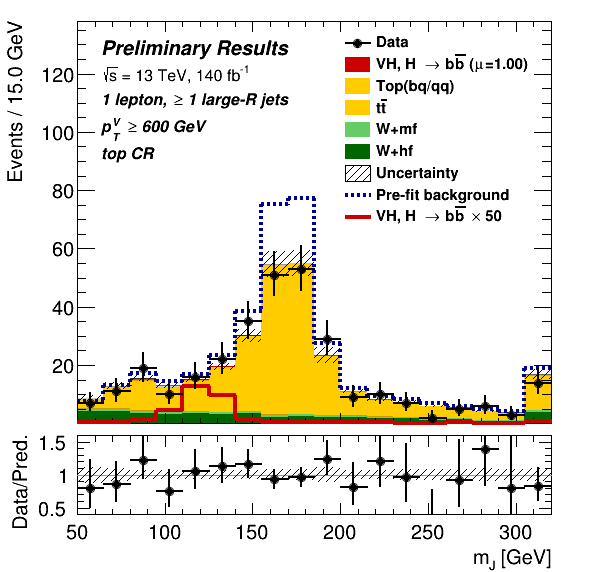
\includegraphics[width=0.32\textwidth]{Images/VH/Own_fit/postfit_VHbb/Region_distmBB_BMin600_incFat1_Fat1_DSRtopaddbjetcr_J0_TTypebb_incJet1_T2_L1_Y6051_GlobalFit_conditionnal_mu1.png}
        \caption{The \ptv\ $\in$ [400, 600] GeV (left) and \ptv\ $\geq$ 600 GeV (right) boosted Top CR.}
        \label{fig:plots_VHbbBoost_1L_topCR}
    \end{subfigure}
    \caption{The boosted $BB$-tagged 0L regions.}
    \label{fig:plots_VHbbBoost_1L}
\end{figure} 

% 2L
\vspace*{\fill}

\begin{figure}[h!]
    \centering
    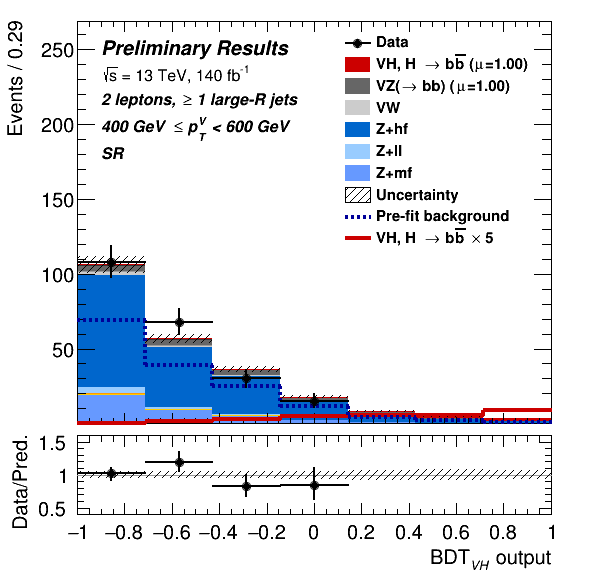
\includegraphics[width=0.32\textwidth]{Images/VH/Own_fit/postfit_VHbb/Region_distmva_BMax600_BMin400_incFat1_Fat1_DSR_J0_TTypebb_incJet1_T2_L2_Y6051_GlobalFit_conditionnal_mu1.png}
    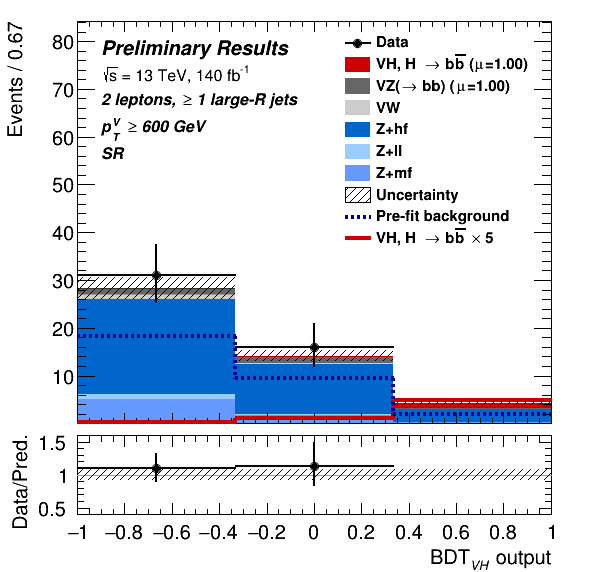
\includegraphics[width=0.32\textwidth]{Images/VH/Own_fit/postfit_VHbb/Region_distmva_BMin600_incFat1_Fat1_DSR_J0_TTypebb_incJet1_T2_L2_Y6051_GlobalFit_conditionnal_mu1.png}
    \caption{The boosted $BB$-tagged 2L signal regions, \ptv\ $\in$ [400, 600] (left) and \ptv\ $\geq$ 600 GeV (right).}
    \label{fig:plots_VHbbBoost_2L_SR}
\end{figure} 
